% -----------------------------------------------------------------
% Document class: Article
\documentclass[ a4paper, twoside, 11pt]{article}
\usepackage{../../../macros-general}
\usepackage{../../../macros-article}
% Number of the handout, quiz, exam, etc.
\newcommand{\numero}{05}
\setcounter{numero}{\numero}

% -----------------------------------------------------------------
\begin{document}
\allowdisplaybreaks

\begin{center}
\Large Mec\'anica Vectorial (MECG-1001): Trabajo Aut\'onomo \numero \\[2ex]
\small \textbf{Semestre:} 2017-2018 T\'ermino II \qquad
\textbf{Instructor:} Luis I. Reyes Castro \qquad
\textbf{Paralelo:} 09
\end{center}
\fullskip

% =============================================
\begin{problem}
\textbf{[4 Puntos]} Cada uno de los engranes $A$ y $B$ pesa 20 lbs y tiene un radio de giro de 7.5 in; el engrane $C$ pesa 5 lb y tiene un radio de giro de 3 in. Si un par $M$ de magnitud constante de 50 lb-in se aplica al engrane $C$, determine \textit{(i)} la aceleraci\'on angular del engrane $A$, \linebreak \textit{(ii)} la fuerza tangencial que ejerce el engrane $C$ sobre el engrane $A$.

\begin{figure}[htb]
\centering
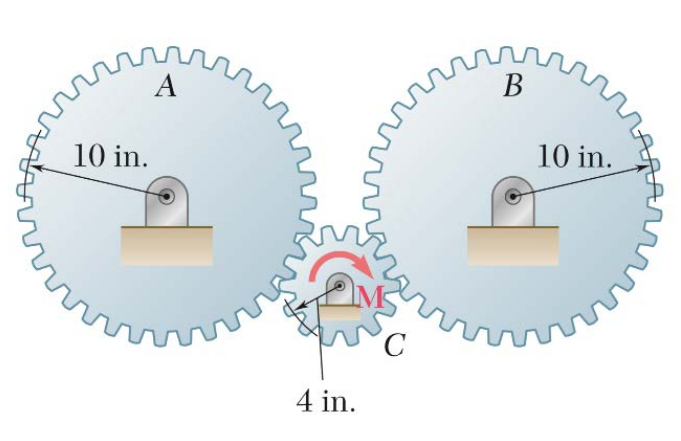
\includegraphics[width=0.4\textwidth]{problema-1.jpg}
\end{figure}

\emph{Soluci\'on:} Primero calculamos los momentos de inercia y el torque externo: 
\begin{align*}
I_{AB} \; & = \; (20/32.2) \, (7.5/12)^2 \; = \;
0.2426 \; \text{slug - ft\tsup{2}} \\
I_{C} \; & = \; (5/32.2) \, (3/12)^2 \; = \;
0.0097 \; \text{slug - ft\tsup{2}} \\
\vec{M} \; & = \; -4.167 \; \uvec{k} \; \text{lb-ft}
\end{align*}
Luego bosquejamos los diagramas de cuerpo libre (DCL) de los engranes, tal como se muestra en la siguiente fotograf\'ia. 
\begin{figure}[htb]
\centering
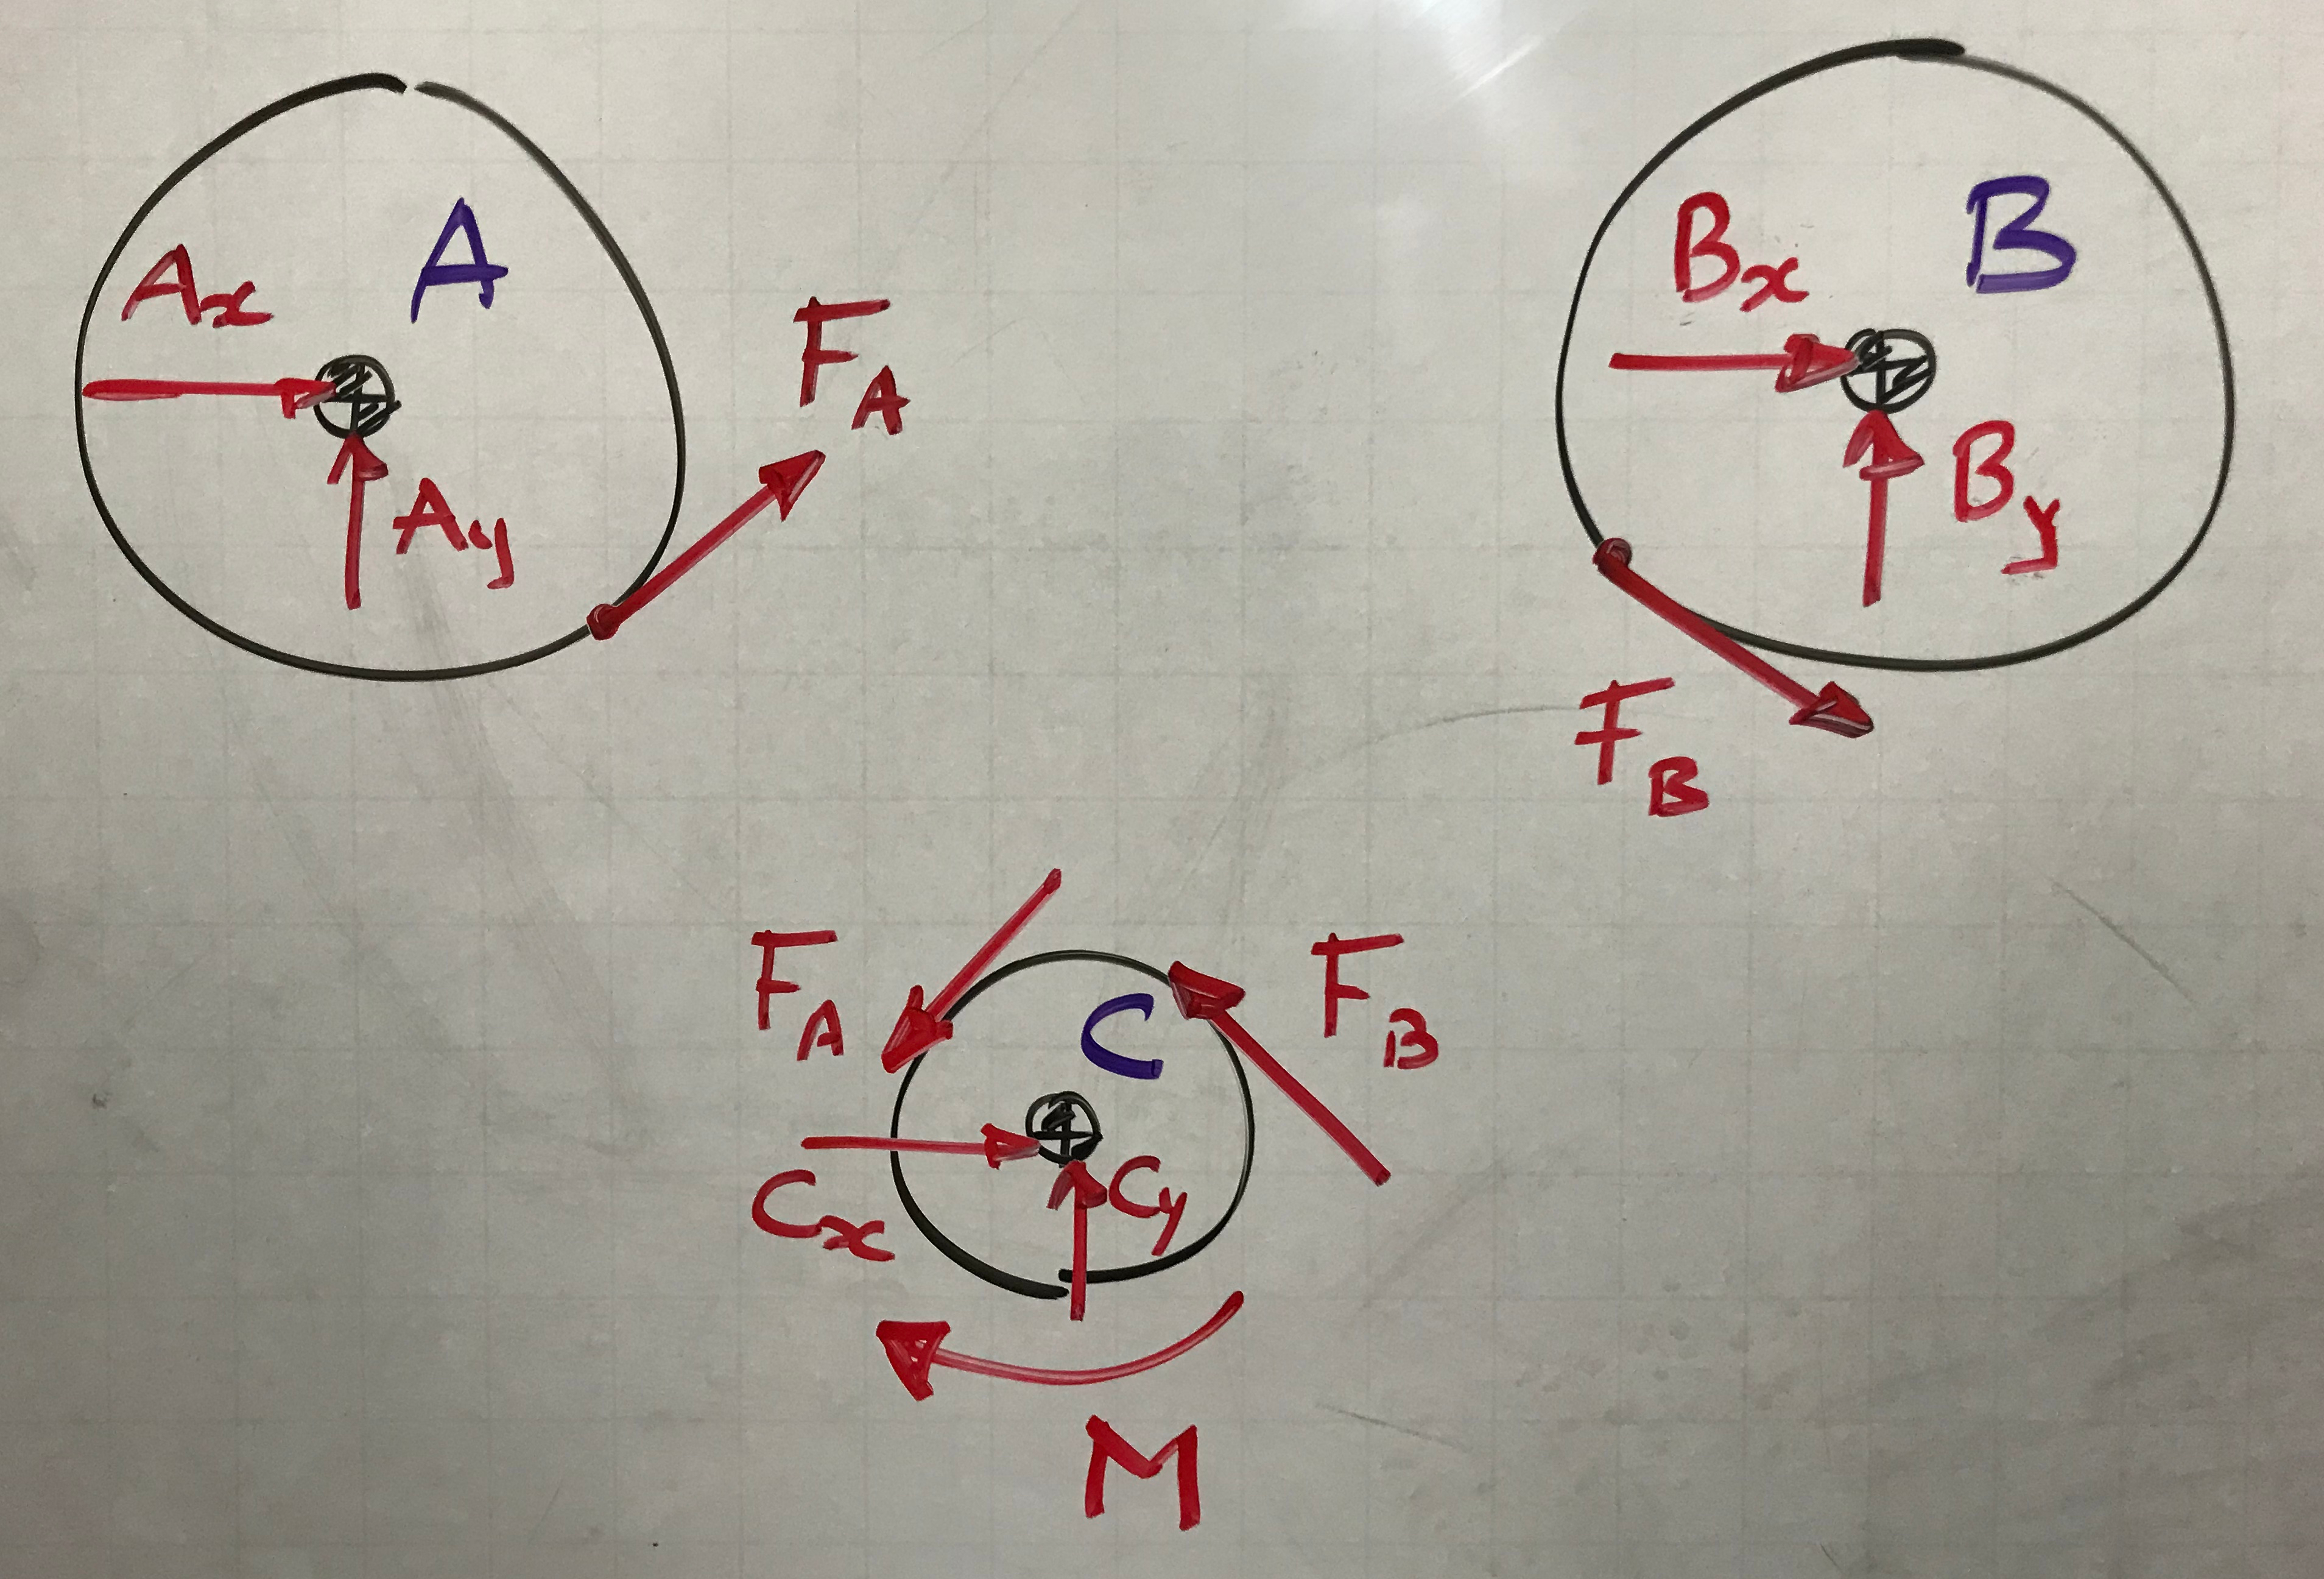
\includegraphics[width=0.5\textwidth]{problema-1_DCL.jpg}
\end{figure}

Tomando las sumatorias de torques externos sobre cada engrane, obtenemos:
\begin{align*}
& +r_{AB} \, F_A \; = \; I_{AB} \, \alpha_A \\
& +r_{AB} \, F_B \; = \; I_{AB} \, \alpha_B \\
& + r_C \, ( F_A + F_B ) - M \; = \; I_C \, \alpha_C
\end{align*}
Ahora tomamos en cuenta la condici\'on de rodadura: 
\[
r_{AB} \, \alpha_A \; = \; -r_C \, \alpha_C \qquad \qquad \qquad
r_{AB} \, \alpha_B \; = \; -r_C \, \alpha_C
\]
Resolviendo para $F_A$ y $F_B$ en las sumatorias de torques externos, obtenemos: 
\[
F_A \; = \; F_B \; = \; -\frac{ I_{AB} \, r_C \, \alpha_C }{r_{AB}^2}
\]
Consecuentemente, la sumatoria de torques en el engrane $C$ resulta en:
\begin{align*}
-2 \, I_{AB} \left( \frac{r_C}{r_{AB}} \right)^2 \alpha_C \; - \; M
\; = \; I_C \, \alpha_C \quad
& \Longrightarrow \;
\alpha_C \; = \; -47.714 \, \uvec{k} \; \text{ rad/s\tsup{2}} \\
& \Longrightarrow \;
\alpha_A \; = \; +19.086 \, \uvec{k} \; \text{ rad/s\tsup{2}}
\end{align*}
Finalmente, la fuerza tangencial deseada es: 
\[
F_A \; = \; F_B \; = \; 5.556 \; \text{lbs}
\]
\QED

\end{problem}
\fullskip

% =============================================
\begin{problem}
\textbf{[4 Puntos]} Una barra ligera de 1.5 kg est\'a soldada a un disco uniforme de 5 kg en la forma que se muestra. El ensamble oscila libremente alrededor de $C$ en un plano vertical. Si en la posici\'on indicada el ensamble es liberado con una velocidad angular de 10 rad/s \linebreak en direcci\'on de las manecillas del reloj, determine \textit{(i)} la aceleraci\'on angular del ensamble, \linebreak \textit{(ii)} las componentes de la reacci\'on en $C$. 

\begin{figure}[htb]
\centering
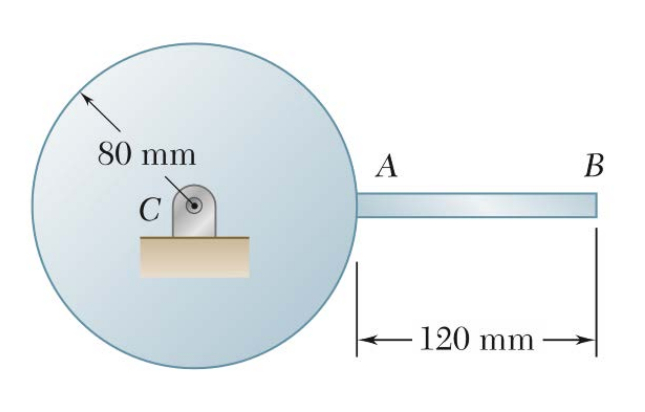
\includegraphics[width=0.4\textwidth]{problema-2.jpg}
\end{figure}

\emph{Soluci\'on:} Primero localizamos el centro de masa del ensamble. Para esto ubicamos el origen del sistema de referencia en $C$ y definimos al centro de masa como $\vec{r_G} = r_G \, \uvec{i}$. Entonces: 
\[
r_G \; = \; \frac{(5)(0) + (1.5)(0.140)}{5+1.5} \; = \;
0.0323 \; \text{m} \quad \Longrightarrow \quad
\vec{r_G} \; = \; 0.0323 \, \uvec{i} \; \text{m}
\]
Despu\'es calculamos su momento de inercia utilizando el Teorema de Steiner: 
\begin{align*}
I \;
& = \; (1/2)(5)(0.080)^2 + (5)(0.0323)^2 + (1/12)(1.5)(0.120)^2 + (1.5)(0.140-0.0323)^2 \\
& = \; 0.0404 \; \text{kg - m\tsup{2}}
\end{align*}
Luego bosquejamos el diagrama de cuerpo libre (DCL) del ensamble, tal como se muestra en la siguiente fotograf\'ia. 
\begin{figure}[htb]
\centering
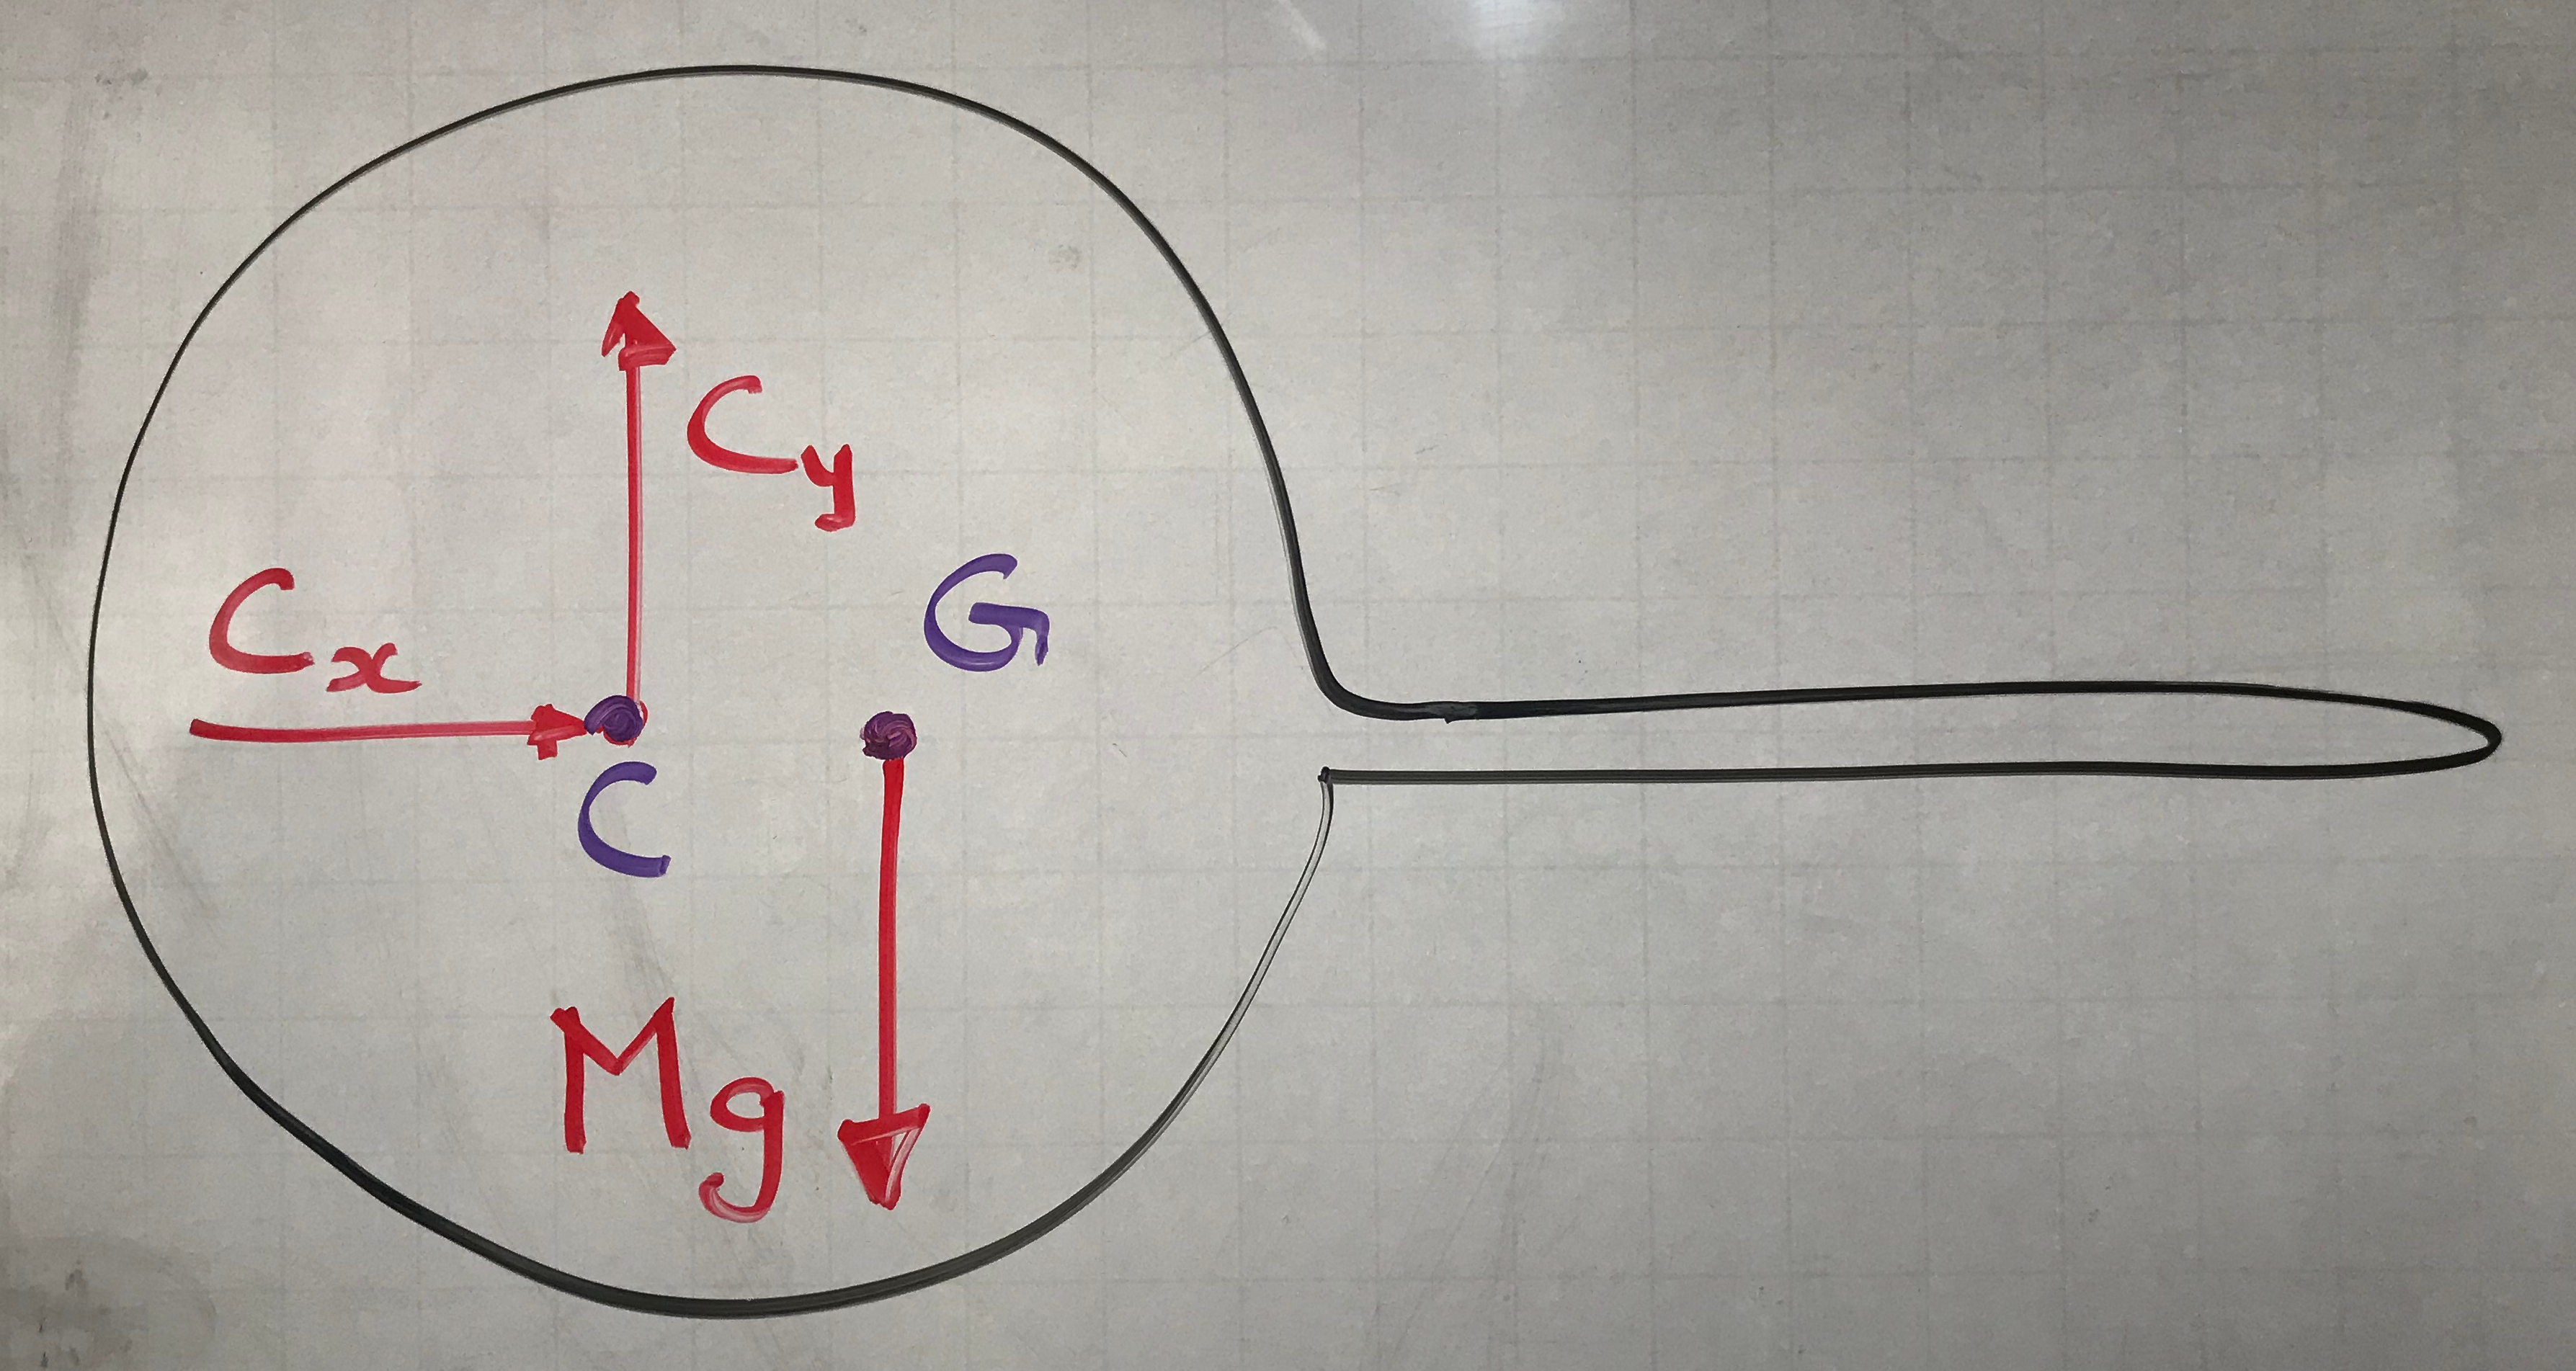
\includegraphics[width=0.5\textwidth]{problema-2_DCL.jpg}
\end{figure}

Entonces, las sumatorias de fuerzas y torques externos son: 
\begin{align*}
M \, (\vec{a_G})_x \; & = \; C_x \\
M \, (\vec{a_G})_y \; & = \; C_y - M g \\
I \, \alpha \; & = \; -r_G \, C_y
\end{align*}
Ahora debemos relacionar $\vec{a_G}$ con $\alpha$ utilizando restricciones cinem\'aticas. Recordando que la velocidad angular del ensamble es $\vec{\omega} = -10 \, \uvec{k}$ rad/s, vemos que: 
\begin{align*}
\vec{a_G} \; & = \;
\vec{a_C} + \vec{\alpha} \cross \vec{r_{CG}} + 
\vec{\omega} \cross ( \vec{\omega} \cross \vec{r_{CG}} ) \\
\; & = \;
\vec{0} + \vec{\alpha} \cross \vec{r_{G}} - \omega^2 \, \vec{r_G} \\
\; & = \; -100 \, r_G \, \uvec{i} + r_G \, \alpha \, \uvec{j} \; \text{ft/s\tsup{2}}
\end{align*}
En vista de que $(\vec{a_G})_x = -100 \, r_G$, de la sumatoria de fuerzas extenas en $x$ obtenemos: 
\[
C_x \; = \; -100 \, r_G \, M \; = \; -21.0 \, \text{N}
\]
Puesto que $(\vec{a_G})_y = +r_G \, \alpha$, la sumatoria de fuerzas extenas en $y$, junto con la sumatoria de torques externos, nos proveen de un sistema de dos ecuaciones en dos inc\'ognitas: 
\begin{align*}
M \, r_G \, \alpha \; & = \; C_y - M g \\
I \, \alpha \; & = \; -r_G \, C_y
\end{align*}
Resolviendo dicho sistema, obtenemos $\alpha = -43.65$ rad/s\tsup{2} y $C_y = +54.6$ N. En conclusi\'on: 
\[
\vec{\alpha} \; = \; -43.65 \, \uvec{k} \; \text{rad/s\tsup{2}} \qquad
\vec{C} \; = \; ( \, -21.0, \, +54.6 \, ) \; \text{N}
\]


\end{problem}
\fullskip

\end{document}